\section{Lecture 3: The Action Principle and the Calculus of Variations}

We begin by considering \textbf{Fermat's principle}, which governs the path of light.

\begin{definition}[Fermat's Principle]
    Light travels along the path that minimizes the travel time between two points.
\end{definition}

This can also be expressed by stating that light follows a path that minimizes the 
optical path length, given by 

\begin{equation}
    L = \int ds \sqrt{\left(\frac{dx}{ds}\right)^2 + \left(\frac{dy}{ds}\right)^2}.
    \label{eq:optical_path_length}
\end{equation}

This principle demonstrates that light minimizes a particular quantity along its 
trajectory. This naturally leads us to ask: does a similar principle apply to the 
trajectories of mechanical systems?  The answer is yes.

Consider all possible paths $q_i(t)$ that a mechanical system could take through 
configuration space. For a given path, we define the \textbf{action} of the path, denoted 
by $S[q_i(t)]$, as:

\begin{equation}
    S[q_i(t)] = \int_{t_{\text{initial}}}^{t_{\text{final}}} L(q_i, \dot{q}_i, t) \, dt
    \label{eq:action_definition}
\end{equation}

where $L$ is the Lagrangian of the system.  It turns out that the path that a mechanical
system actually takes through configuration space is the one that \textbf{extremizes} the 
action. This is known as the \textbf{Principle of Least Action} or 
\textbf{Hamilton's Principle}. The action $S[q_i(t)]$ is a \textit{functional}, which is 
a function of a function. We denote functionals using square brackets, e.g., $S[f]$, to 
distinguish them from functions like $f(x)$.

In standard calculus, we minimize functions of a finite number of variables. Here, we 
are tasked with minimizing a \textit{functional}, which depends on an entire curve. 
This requires a new set of tools, which fall under the domain of the 
\textbf{Calculus of Variations}.

To understand this, let's consider a general problem. Suppose we have a function 
$F(y(x), y^\prime(x), x)$, and we want to minimize the functional:

\begin{equation}
    I[y(x)]=\int_{x_{0}}^{x_{1}} F(y(x), y'(x), x) \, dx
\end{equation}

where $y(x)$ is defined on the interval $x_0 \leq x \leq x_1$ and $y'(x) = \frac{dy}{dx}$. 
The goal is to find the function $y(x)$ that extremizes $I[y(x)]$.

We proceed as follows:

\begin{itemize}
    \item Fix the values of $y(x_0)$ and $y(x_1)$.
    \item Consider a curve $y(x)$ connecting these endpoints.
    \item Introduce a small perturbation to this curve: $y(x) \rightarrow y(x) + \delta y(x)$.
    \item Compute the variation $\delta I$ due to this perturbation, and require that the term linear in $\delta y$ vanishes.
    \item Since we have fixed the endpoints, we require $\delta y(x_0) = \delta y(x_1) = 0$.
\end{itemize}

\begin{figure}[ht]
    \centering
    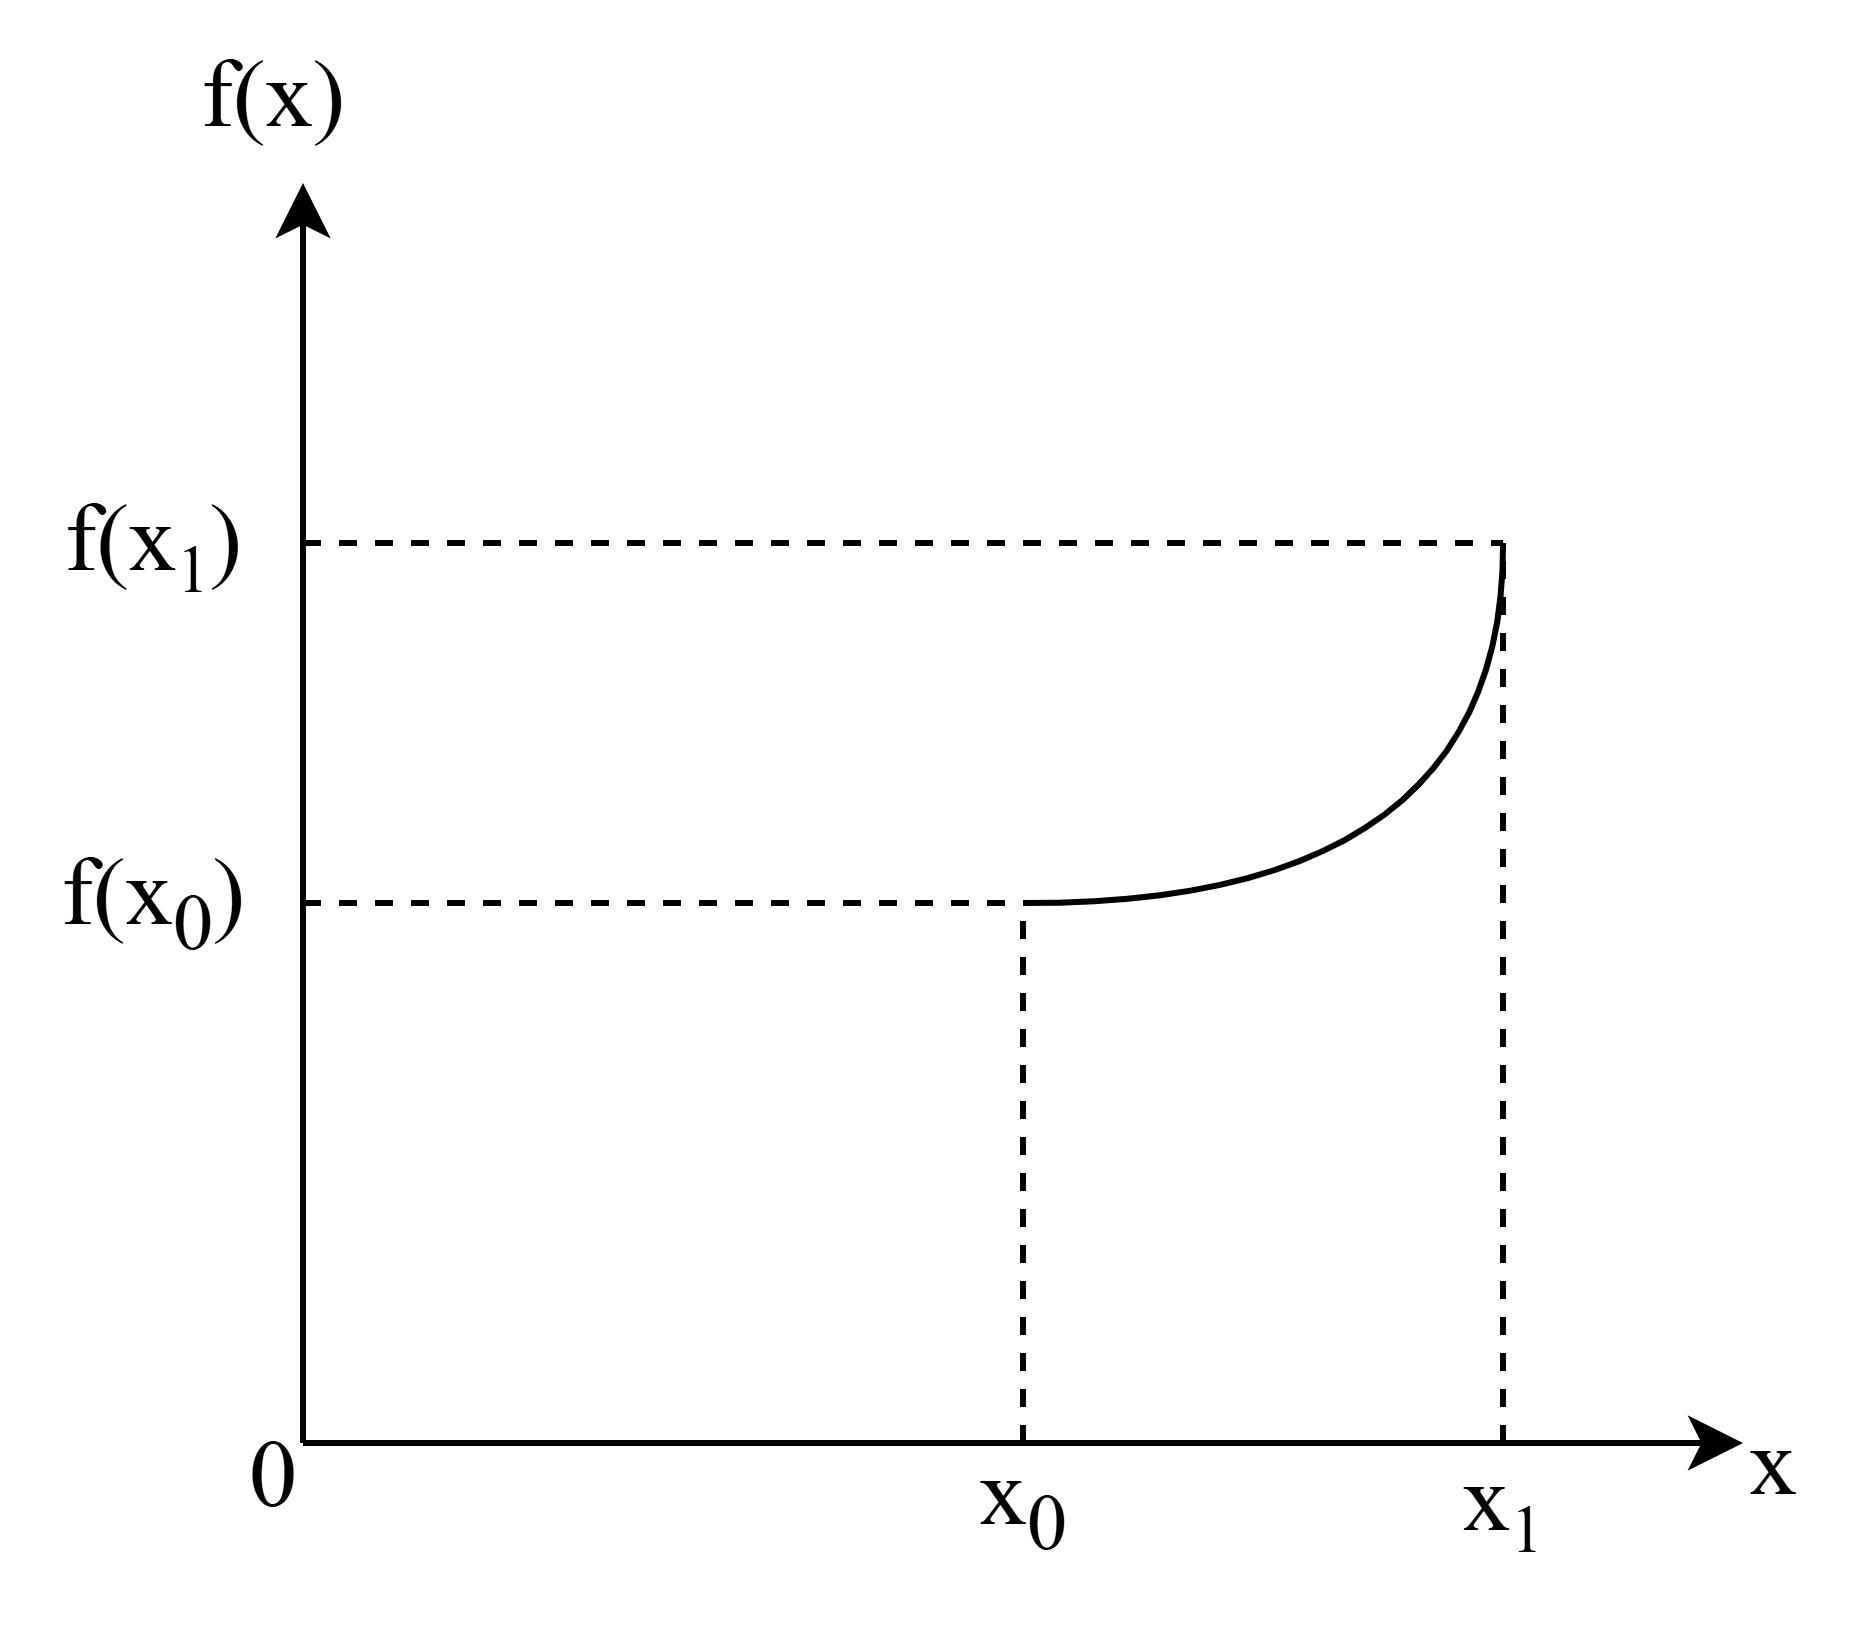
\includegraphics[width=0.4\textwidth]{images/3-1-1.png}
    \caption{Calculus of Variations: Varying a Curve}
    \label{fig:3-1-1}
\end{figure}

The change in the functional due to the perturbation is:

\begin{equation}
    \delta I = I[y(x) + \delta y(x)] - I[y(x)] = \int_{x_0}^{x_1} \left( F(y + \delta y, y' + \delta y', x) - F(y, y', x) \right) dx
    \label{eq:delta_I_definition}
\end{equation}

Using a first-order Taylor expansion of $F$, we have:

\begin{align}
    \delta I &\approx \int_{x_0}^{x_1} dx \left( \frac{\partial F}{\partial y} \delta y + \frac{\partial F}{\partial y'} \delta y' \right)
\end{align}

Note that $\delta y' = \frac{d}{dx}(\delta y)$. Integrating the second term by parts 
(with $u = \frac{\partial F}{\partial y'}$ and $dv = \frac{d}{dx}(\delta y)\, dx$), and 
using the fact that $\delta y(x_0) = \delta y(x_1) = 0$, we get:

\begin{align}
    \delta I &= \int_{x_0}^{x_1} dx \left( \frac{\partial F}{\partial y} \delta y - \frac{d}{dx} \left(\frac{\partial F}{\partial y'}\right) \delta y \right)
\end{align}

Combining the terms, we obtain:

\begin{equation}
    \delta I = \int_{x_0}^{x_1} dx \left( \frac{\partial F}{\partial y} - \frac{d}{dx} \left(\frac{\partial F}{\partial y'}\right) \right) \delta y
\end{equation}

For $\delta I$ to be zero for an arbitrary perturbation $\delta y(x)$, the term inside 
the parentheses must vanish, giving us the \textbf{Euler-Lagrange Equation}:

\begin{equation}
    \frac{\partial F}{\partial y} - \frac{d}{dx} \left(\frac{\partial F}{\partial y'}\right) = 0
\end{equation}

The quantity

\begin{equation}
    \frac{\delta I}{\delta y(x)} = \frac{\partial F}{\partial y} - \frac{d}{dx} \left(\frac{\partial F}{\partial y'}\right)
\end{equation}

is called the \textbf{functional derivative} of $I[y(x)]$ with respect to $y(x)$.

The above result can be easily generalized to a functional that depends on $N$ functions
$y_i(x)$, rather than just one:

\begin{equation}
    I[y_i(x)] = \int dx F(y_i, \frac{dy_i}{dx}, x), \quad i = 1, 2, \dots, N
    \label{eq:functional_multiple_functions}
\end{equation}

Following the same procedure as before, we obtain the condition for extremizing $I$:

\begin{equation}
    \frac{\delta I}{\delta y_i} = \frac{\partial F}{\partial y_i} - \frac{d}{dx} \left(\frac{\partial F}{\partial y'_i}\right) = 0
\end{equation}

This Euler-Lagrange equation must hold for all $i$.

In the context of mechanics, we have that the action is defined as 
$S[q_i(t)] = \int L\ dt$, where $L\left(q_i, \dot{q_i}, t\right)$ is the Lagrangian. Thus,
 the extremization of the action implies the following Euler-Lagrange equations:

\begin{equation}
    \frac{\delta S}{\delta q_i} = \frac{\partial L}{\partial q_i} - \frac{d}{dt} \left(\frac{\partial L}{\partial \dot{q}_i}\right) = 0
\end{equation}

These are the equations of motion for the system.

Let us apply the calculus of variations to an elementary problem.

\begin{example}
    Prove that the shortest distance between two points is a line.
\end{example}

\begin{proof}
    The length of the path can be written as:
    \begin{equation}
        L = \int ds \sqrt{\left(\dot{x}^2 + \dot{y}^2\right)}
    \end{equation}
    Here $\dot{x}$ represents $\frac{dx}{ds}$.
    The Euler-Lagrange equations give us:
    \begin{align}
        \frac{\delta L}{\delta x\left(s\right)} &= -\frac{d}{ds} 
        \left(\frac{\dot{x}}{\sqrt{\dot{x}^2 + \dot{y}^2}}\right) = 0
    \end{align}
    This can be simplified to:
    \begin{equation}
       \frac{d}{ds} \left(\frac{\dot{x}}{\sqrt{\dot{x}^2 + \dot{y}^2}}\right) = 0
       \label{eq:euler_lagrange_shortest_x}
    \end{equation}
    Similarly, for y we get
    \begin{equation}
       \frac{d}{ds} \left(\frac{\dot{y}}{\sqrt{\dot{x}^2 + \dot{y}^2}}\right) = 0
    \end{equation}

    From equation \eqref{eq:euler_lagrange_shortest_x} we can get:
    \begin{equation}
        \frac{\ddot{x}}{\dot{x}} = \frac{\ddot{y}}{\dot{y}}
    \end{equation}
    \begin{equation}
        \frac{d}{ds} \left(\log \dot{x}\right) = \frac{d}{ds} \left(\log \dot{y}\right)
    \end{equation}
    which means:
    \begin{equation}
        \frac{d}{ds} \log \frac{\dot{x}}{\dot{y}} = 0
    \end{equation}
    i.e.,
    \begin{equation}
        \frac{dx}{dy} = \text{constant}
    \end{equation}
    Thus the shortest path between two points is a line.
\end{proof}

We have found that
\begin{equation}
    p_x = \frac{\partial L}{\partial \dot{x}} = \frac{\dot{x}}{\sqrt{\dot{x}^2 + \dot{y}^2}} = \text{const}
\end{equation}

Likewise, 

\begin{equation}
    p_y = \frac{\dot{y}}{\sqrt{\dot{x}^2 + \dot{y}^2}} = \text{const}
\end{equation}

So we can get: 

\begin{equation}
    \frac{p_x}{p_y} = \frac{\dot{x}}{\dot{y}} = \text{const}
\end{equation}

This shows that $\frac{dx}{dy}$ is constant, which implies a straight line. Also, the 
quantities $p_x$ and $p_y$ are constants of motion.